\documentclass[english,aspectratio=43,t]{beamer}
% useful options:
%   aspectratio=169

\usepackage[utf8]{inputenc}
\usepackage{babel}
\usepackage{fixltx2e}
\usepackage{graphicx}
\usepackage{longtable}
\usepackage{float}
\usepackage{wrapfig}
\usepackage{soul}
\usepackage{textcomp}
\usepackage{marvosym}
\usepackage{latexsym}
\usepackage{amsfonts,amsmath,amssymb,amsthm} 
\usepackage{wasysym}
\usepackage{hyperref}
\usepackage{mathtools}
\tolerance=1000
\usepackage{listings}
\usepackage[iso]{isodate}
\usepackage[backend=biber]{biblatex}

\usepackage{bytefield}						% Bytefield
\usepackage{moeptikz}						% tikz-packages for networking symbols
\usepackage{tikz}							% tikz-figures
\usetikzlibrary{decorations.pathreplacing,positioning,arrows,automata}
\tikzstyle{line} = [draw,thick,-latex]
\tikzstyle{transition} = [font=\small]

% select theme before using any of its features
\usetheme{Comsys}
\addbibresource{references.bib}

% data for figure
\begin{filecontents}{tcp.data}
#Transmission round		Congestion Window Size
1		1
2		2
3		4
4		8
5		16
6		32
7		16
8		17
9		18
10		19
11		20
12		10
13		5
14		6
15		7
\end{filecontents}


\title[Cool]{The Origins of Congestion\\and Network-assisted end-to-end\\Congestion Control}
\author{Til Mohr}
\authorextra{Advisor: Jan Rüth}
%\subtitle{Proseminar}
\date{\today}
%\location{Aachen}
%\projectlogo[scale=0.5]{logos/rwth_comsys_cropped}
%\logoextra{logos/rwth_comsys_cropped}

%\titlegraphics{images/presentation}
%\begin{titlepicture}
%	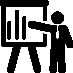
\includegraphics[width=3cm]{images/presentation}
%\end{titlepicture}


\begin{document}


\titleframe


\begin{frame}
	\frametitle{Outline}
	\tableofcontents
\end{frame}

\section{Introduction}
\label{sec:intro}
\AtBeginSection[]
{
  \begin{frame}
	\frametitle{Outline}
    \tableofcontents[currentsection]
  \end{frame}
}

\begin{frame}{Introduction}
  \nocite{*}
\begin{columns}
	\begin{column}{.5\textwidth}
		\only<1>{
		\begin{figure}
		\centering
		\begin{tikzpicture}
			\node [client, scale=0.7] (Client1) {};
			\node [router, scale=0.7] (Router1) [below right = 0.35cm and 2cm of Client1] {};
			\node [server, scale=0.7] (Server1) [above right = 0.35cm and 2cm of Router1] {};
			\node [router, scale=0.7] (Router2) [below right = 2cm and 0.75cm of Client1] {};
			\node [router, scale=0.7] (Router3) [right = 2.25cm of Router2] {};
			\node [server, scale=0.7] (Server2) [below left = 1.75cm and -0.1cm of Router2] {};
			\node [client, scale=0.7] (Client2) [below right = 1.75cm and 0.1cm of Router3] {};
					
			\draw[-] (Client1) -- (Router2);
			\draw[-] (Router1) -- (Router2);
			\draw[-] (Server1) -- (Router1);
			\draw[-] (Router1) -- (Router3);
			\draw[-] (Router2) -- (Server2);
			\draw[-] (Router3) -- (Server2);
			\draw[-] (Router3) -- (Client2);
		\end{tikzpicture}
		\end{figure}
		}
		
		\only<2->{
		\begin{figure}
		\centering
		\begin{tikzpicture}
			\node[state, scale=0.7] (Client1) {};
			\node[state, scale=0.7] (Router1) [below right = 0.35cm and 2cm of Client1] {};
			\node[state, scale=0.7] (Server1) [above right = 0.35cm and 2cm of Router1] {};
			\node[state, scale=0.7] (Router2) [below right = 2cm and 0.75cm of Client1] {};
			\node[state, scale=0.7] (Router3) [right = 2.25cm of Router2] {};
			\node[state, scale=0.7] (Server2) [below left = 1.75cm and -0.1cm of Router2] {};
			\node[state, scale=0.7] (Client2) [below right = 1.75cm and 0.1cm of Router3] {};
			
			\only<2>{
			\draw[-] (Client1) -- (Router2);
			\draw[-] (Router1) -- (Router2);
			\draw[-] (Server1) -- (Router1);
			\draw[-] (Router1) -- (Router3);
			\draw[-] (Router2) -- (Server2);
			\draw[-] (Router3) -- (Server2);
			\draw[-] (Router3) -- (Client2);
			}
			\only<3->{
			\path
				(Client1) edge [left] node [transition] {10} (Router2)
				(Router1) edge [above left] node [transition] {3} (Router2)
				(Server1) edge [above] node [transition] {25} (Router1)
				(Router1) edge [below left] node [transition] {30} (Router3)
				(Router2) edge [left] node [transition] {9} (Server2)
				(Router3) edge [below right] node [transition] {28} (Server2)
				(Router3) edge [left] node [transition] {13} (Client2)
			;
			}
		\end{tikzpicture}
		\end{figure}
		}
	\end{column}
	
	\only<1-2>{\begin{column}{.45\textwidth}\end{column}}
	\only<3->{
	\begin{column}{.45\textwidth}
		\begin{itemize}
		\item Links have limitations.
		\item<4-> Data is split up into smaller packets.
		\item<5-> Network nodes contain buffers storing packets.
		\end{itemize}
		\only<5->{
		\begin{alertblock}{}
		Origins of Congestion are versatile.
		\end{alertblock}
		}
	\end{column}
	}
\end{columns}
\end{frame}

\section{Origins of Congestion}
\label{sec:oc}
\AtBeginSection[]
{
  \begin{frame}
	\frametitle{Outline}
    \tableofcontents[currentsection]
  \end{frame}
}

\subsection{Buffers}
\label{sec:buffers}
\begin{frame}{Buffers}
~\\
\begin{block}{Purpose}
Buffers store packets in network nodes waiting for transmission.
\end{block}
~\\
\only<2->{
Sizing Buffers:
\begin{itemize}
\item Buffer size should be large enough to handle packet bursts.
\item Too large buffers result in an increase of queuing delay and \textit{over-buffering}.
\end{itemize}
}
~\\
\only<3->{
\begin{enumerate}
\item[$\Rightarrow$] Buffers should be designed according to their application environment.
\end{enumerate}
}
\end{frame}

\begin{frame}{Bufferbloat}
\begin{itemize}
\item Refers to frequently full, excessively large buffers.
\item<2-> Queued packets will not be dropped, resulting in:
\only<2->{
	\begin{itemize}
	\item Unnecessary network delay (\textit{latency}) and packet delay fluctuation (\textit{jitter}).
	\item Increased congestion, as TCP is not being notified of congestion.
	\item Decreases network throughput.
	\end{itemize}
}
\item<3-> With memory getting cheaper over the years, buffers saw an increase in size.
\end{itemize}
\end{frame}

\subsection{Delay}
\label{sec:delay}
\begin{frame}{Delay}
~\\
\centering
\begin{figure}
\centering
	\begin{tikzpicture}
		\node (net1) {};
		\node[router, scale=0.8] (Router1) [right = 1.5cm of net1] {};
		\node[router, scale=0.8] (Router2) [right = 3.2cm of Router1] {};
		\node[router, scale=0.8] (Router3) [right = 3.2cm of Router2] {};
		\node (net2) [right = 1.5cm of Router3] {};
		
		\draw[-, dotted] (net1) -- (Router1);
		\draw[-] (Router1) -- (Router2);
		\draw[-] (Router2) -- (Router3);
		\draw[-, dotted] (Router3) -- (net2);
	\end{tikzpicture}
\end{figure}
~\\
\begin{minipage}{\textwidth}
\begin{columns}
%Content
\only<2->{
	\begin{column}{0.5\textwidth}
		\begin{block}{Transmission Delay}
			Depends on bandwidth and length of the connection.
		\end{block}
	\end{column}
}
\only<3->{
	\begin{column}{0.5\textwidth}
		\begin{block}{Processing Delay}
			Time it takes to process a single packet.
		\end{block}
	\end{column}
}
%Placeholders
\only<1>{\begin{column}{0.5\textwidth}\end{column}}
\only<1-2>{\begin{column}{0.5\textwidth}\end{column}}
\end{columns}
\end{minipage}

\begin{minipage}{\textwidth}
\begin{columns}
\only<4->{
	\begin{column}{0.5\textwidth}
		\begin{block}{Inter-Packet Delay}
			Allows the receiver to prepare for transmission.
		\end{block}
	\end{column}
}
\only<5->{
	\begin{column}{0.5\textwidth}
		\begin{block}{Queuing Delay}
			Time a packet waits in the buffer waiting for transmission.
		\end{block}
	\end{column}
}
\only<1-3>{\begin{column}{0.5\textwidth}\end{column}}
\only<1-4>{\begin{column}{0.5\textwidth}\end{column}}
\end{columns}
\end{minipage}
\end{frame}

\subsection{Overview over Congestion}
\label{sec:ooc}

\begin{frame}{Overview over Congestion}
\begin{columns}
\begin{column}{0.5\textwidth}
	\begin{block}{Buffers}
		\begin{itemize}
		\only<2->{\pgfsetfillopacity{0.2}}
		\item Buffer size
		\only<2->{\pgfsetfillopacity{1}}
		\item Buffer management
		\end{itemize}
	\end{block}
\end{column}

\begin{column}{0.5\textwidth}
	\begin{block}{Delay}
		\begin{itemize}
		\only<2->{\pgfsetfillopacity{0.2}}
		\item Transmission Delay
		\item Processing Delay
		\item Inter-Packet Delay
		\only<2->{\pgfsetfillopacity{1}}
		\item Queuing Delay
		\end{itemize}
	\end{block}
\end{column}
\end{columns}
~\\~\\
\only<2->{
\begin{itemize}
\item Congestion control algorithms can improve queuing delay, number of queued packets and buffer management.
\end{itemize}
}
\end{frame}

\section{TCP Congestion Avoidance}
\label{sec:ca}
\AtBeginSection[]
{
  \begin{frame}
	\frametitle{Outline}
    \tableofcontents[currentsection]
  \end{frame}
}

\begin{frame}{TCP}
~\\
\begin{block}{Transmission Control Protocol}
\begin{itemize}
\item Lives on transport layer, communicates with application layer via sockets ($\rightarrow$ ports) and uses IP as internet protocol ($\rightarrow$ TCP/IP).
\item Ensures successful transmission of all data.
\end{itemize}
\end{block}
\begin{itemize}
\item<2-> Transmitted data needs to be acknowledged.
\item<2-> Adjusts to the current state of congestion.
\item<3-> Many different implementations exist.
\end{itemize}
\end{frame}

\begin{frame}[fragile]{TCP Header}
\centering
\begin{figure}
\centering
\begin{bytefield}[bitheight=2.2\baselineskip, bitwidth=0.635\baselineskip]{32}
\bitbox{16}{Source Port} & \bitbox{16}{Destination Port} \\
\bitbox{32}{Sequence Number} \\
\bitbox{32}{Acknowledgment Number} \\
\bitbox{4}{Data Offset} & \bitbox{4}{Rsrvd} & \bitbox{1}{\tiny C\\W\\R} & \bitbox{1}{\tiny E\\C\\E} & \bitbox{1}{\tiny U\\R\\G} & \bitbox{1}{\tiny A\\C\\K} & \bitbox{1}{\tiny P\\S\\H} & \bitbox{1}{\tiny R\\S\\T} & \bitbox{1}{\tiny S\\Y\\N} & \bitbox{1}{\tiny F\\I\\N} & \bitbox{16}{Window Size} \\
\bitbox{16}{Checksum} & \bitbox{16}{Urgent Pointer} \\
\bitbox{32}{Options} \\
\bitbox{32}{Data}
\end{bytefield}
\end{figure}
\end{frame}

\subsection*{Perceiving Congestion}
\label{sec:pc}

\begin{frame}{Perceiving Congestion}
\begin{columns}
\begin{column}{0.5\textwidth}
\begin{block}{Round-trip Time (\textit{RTT})}
Describes the amount of time between sending a data packet and receiving its acknowledgment packet.
\end{block}
\end{column}
\begin{column}{0.5\textwidth}
\begin{block}{Retransmission Timeout (\textit{RTO})}
The maximum amount of time the sender will wait for the acknowledgment of a packet.
\end{block}
\end{column}
\end{columns}
~\\
\only<2->{
\begin{itemize}
\item Classic TCP perceives congestion by detecting packet loss.
\item Other implementations also perceive congestion by determining variations in RTT over time.
\end{itemize}
}
\end{frame}

\begin{frame}[fragile]{Perceiving Packet Loss - Selective Acknowledgments}
\centering
\begin{figure}
\centering
\begin{tikzpicture}
	\node (Sender) {Sender};
	\node (Receiver) [right = 5cm of Sender] {Receiver};
	\node (s1) [below = 0.5 of Sender] {};
	\node (s2) [below = 0.35cm of s1] {};
	\node (s3) [below = 0.35cm of s2] {};
	\node (r1) [below = 1cm of Receiver] {};
	\node (r2) [below = 0.35cm of r1] {};
	\node (r3) [below = 0.35cm of r2] {};
	\node (r4) [below = 1cm of r3] {};
	\node (r5) [below = 0.35cm of r4] {};
	\node (r6) [below = 0.35cm of r5] {};
	\node (s4) [below = 2cm of s3]  {};
	\node (s5) [below = 0.35cm of s4] {};
	\node (s6) [below = 0.35cm of s5] {};
	\node (Sender2) [below = 1cm of s6] {};
	\node (Receiver2) [below = 1.55cm of r6] {};
	\only<2->{\node (loss) [below right = -0.2cm and 3cm of s2] {\lightning};}
	
	
	\only<1->{\path (s1) edge [above] node {\tiny A} (r1);}
	\only<2->{\path (s2) edge [dashed, above] node {\tiny B} (loss);}
	\only<3->{\path (s3) edge [below] node {\tiny C} (r3);}
	\only<4->{\path (r4) edge [above] node {\tiny A} (s4);}
	\only<5->{\path (r6) edge [above] node {\tiny A} (s6);}
	
	\draw[-] (Sender) -- (Sender2);
	\draw[-] (Receiver) -- (Receiver2);
\end{tikzpicture}
\end{figure}
\end{frame}

\subsection*{Adjusting for Congestion}
\label{sec:ac}
\begin{frame}{Adjusting for Congestion}
~\\
\begin{block}{Goal}
\begin{itemize}
\item Do not fill up buffers in the network.
\item Achieve and hold maximum throughput.
\item Adapt to the current state of congestion as quickly as possible.
\end{itemize}
\end{block}
\only<2->{
\begin{itemize}
\item CA algorithms are based on Additive-Increase Multiplicative-Decrease principle.
\item Variable $cwnd$ (congestion window) describes the maximum amount of data sent before ACKs are needed.
\end{itemize}
}
\end{frame}

\begin{frame}{Adaption - Additive Increase}
~\\
\begin{block}{Formula}
$cwnd \coloneqq cwnd + u$
\end{block}
\begin{itemize}
\item Increases the data rate slowly to reach the networks maximum throughput.
\item Prevents the rapid filling of buffers.
\item Proposed value for $u$: $\frac{1}{cwnd}$
\end{itemize}
\end{frame}

\begin{frame}{Adaption - Multiplicative Decrease}
~\\
\begin{block}{Formula}
$cwnd \coloneqq d \cdot cwnd, 0<d<1$
\end{block}
\begin{itemize}
\item Decreases the data rate drastically.
\item Allows the nodes to recover and buffer lengths to decrease.
\item Proposed value for $d$: $\frac{1}{2}$
\end{itemize}
\end{frame}

\begin{frame}{Adaption - Slow-Start}
~\\
\begin{block}{Formula}
$cwnd \coloneqq cwnd + 1$ for each received ACK packet.
\\$\Rightarrow$ Exponential increase over time.
\end{block}
\begin{itemize}
\item Drastically increases the protocols performance.
\item Used after connection is established or after multiple packet losses have been detected.
\item Switches off after a threshold has been exceeded or congestion has been perceived.
\end{itemize}
\end{frame}

\begin{frame}{Visualization of TCPs Congestion Avoidance}
\centering
\begin{figure}
  \centering
    \begin{tikzpicture}[y=.2cm, x=.5cm]
    	% Ranges and dotted lines
    	\fill[yellow!10]	(0,0) rectangle (6,35);
    	\fill[red!10] 		(6,0) rectangle (7,35);
    	\fill[green!10] 	(7,0) rectangle (11,35);
    	\fill[red!10]		(11,0) rectangle (13,35);
    	\fill[green!10]		(13,0) rectangle (15.3,35);
    	\draw[dotted] 		(6,0) -- (6,35);
    	\draw[dotted] 		(7,0) -- (7,35);
    	\draw[dotted] 		(11,0) -- (11,35);
    	\draw[dotted] 		(13,0) -- (13,35);
    	% Axis
    	\draw[->] 			(0,0) -- coordinate (x axis mid) (17,0);
    	\draw[->] 			(0,0) -- coordinate (y axis mid) (0,35);
    	% Labels
    	\node[below=0.1cm] at (x axis mid) [transition] {Transmission round};
    	\node[rotate=90, above=0.1cm] at (y axis mid) [transition] {Congestion window size};
    	% Plot
    	\draw plot[mark=*]
    		file {tcp.data};
    \end{tikzpicture}
\end{figure}
\end{frame}

\section{Network-assisted Congestion Control}
\label{sec:cc}
\AtBeginSection[]
{
  \begin{frame}
	\frametitle{Outline}
    \tableofcontents[currentsection]
  \end{frame}
}

\begin{frame}{Network-assisted Congestion Control}
\begin{itemize}
\item Congestion Detection algorithms are very implicit:
	\begin{itemize}
	\item Packet loss may also have other causes
	\item Methods are inaccurate, and do not inform about the degree of congestion.
	\end{itemize}
\item[$\Rightarrow$] Creates unnecessary network delay.
~\\~\\
\item<2-> Explicit congestion notification is crucial to keep the network stable.
\item[$\Rightarrow$]<2-> Modify the IP header to include a \textit{Congestion Experienced} Flag (CE).
\item<3-> \textit{Explicit congestion notification} (ECN), an extention to TCP/IP, implements this.
\end{itemize}
\end{frame}

\begin{frame}{Principle of Network-assisted Congestion Control}
\begin{center}
\begin{figure}
	\centering
		\begin{tikzpicture}[->, node distance = 2.1cm]
			%network
			\node[client, scale=0.7] (H1) {};
			\node[router, scale=0.7] (R1) [right=of H1] {};
			\node[router, scale=0.7] (R2) [right=of R1] {};
			\node[router, scale=0.7] (R3) [right=of R2] {};
			\node[client, scale=0.7] (H2) [right=of R3] {};
			\path [line] (H1) -- (R1);
			\path [line] (R1) -- (R2);
			\path [line] (R2) -- (R3);
			\path [line] (R3) -- (H2);
			\path [line, dotted] (H2) -- ++(0,-35pt) -| (H1);
			\node[below=0.9cm of R2] (text) [transition] {Congested Signal};
			
			%packets
			\node[messageclosed,scale=0.5, fill=black!10] (P1) [above right=0.2cm and 1cm of H1] {};
			\node[messageclosed,scale=0.5, fill=black!50] (P2) [above left=0.7cm and 0.3cm of R2] {};
			\node[messageclosed,scale=0.5, fill=black!10] (P3) [above left=0.4cm and 0.2cm of R2] {};
			\node[messageclosed,scale=0.5, fill=black!10] (P4) [above left=0.1cm and 0.1cm of R2] {};
			\node[messageclosed,scale=0.5, fill=black!50] (P5) [above right=0.2cm and 1cm of R3] {};
			\node[above left = 1.5cm and 0cm of R1] (P) [transition] {Packet};
			\node[above right = 1.5cm and -0.3cm of R2] (CN) [transition] {Congested Node};
			\node[above left = 1.5cm and -0.4cm of H2] (MP) [transition] {Marked Packet};
			\path [line] (P) -- (P1);
			\path [line] (CN) -- (R2);
			\path [line] (MP) -- (P5);
		\end{tikzpicture}
\end{figure}
\end{center}
\end{frame}

\subsection{XCP}
\label{sec:xcp}
\begin{frame}{XCP}
~\\
\begin{block}{XCP}
\textit{eXplicit Congestion Protocol} generalizes the ECN proposal.
\end{block}
\begin{itemize}
\item Improves upon ECN by introducing new packet control concepts.
\item Additionally gives feedback about the degree of congestion.
\end{itemize}
\only<2->{
\begin{block}{XCP Header}
\begin{itemize}
\item $H\_cwnd$
\item $H\_rtt$
\item $H\_feedback$
\end{itemize}
\end{block}
}
\end{frame}

\begin{frame}{XCP Sender}
\begin{itemize}
\item As a TCP Sender, the XCP sender also keeps track of $cwnd$ and $RTT$ and deals with packet loss (retransmission).
~\\~\\
\item On data packet depature, the XCP sender will:
	\begin{itemize}
	\item $H\_cwnd \coloneqq cwnd$
	\item $H\_rtt \coloneqq RTT$
	\item $H\_feedback \coloneqq \frac{r \cdot RTT - cwnd}{cwnd}$, where $r$ is the desired data rate.
	\end{itemize}
\item[$\Rightarrow$] The desired data rate can be reached in just one RTT.
~\\~\\
\item On ACK packet arrival, the XCP sender will adjust $cwnd$ according to the received feedback:
	\begin{itemize}
	\item $cwnd \coloneqq max(cwnd + H\_feedback, s)$, where $s$ is the packet size.
	\end{itemize}
\end{itemize}
\end{frame}

\begin{frame}{XCP Router}
\begin{columns}
\begin{column}{.5\textwidth}
\begin{block}{Efficiency Controller (EC)}
\begin{itemize}
\item Maximizes link utilization.
\item Minimizes queue lengths and packet drops.
\item If the node is congested, feedback should be negative, otherwise positive.
\end{itemize}
\end{block}
\end{column}

\begin{column}{.5\textwidth}
\only<2->{
\begin{block}{Fairness Controller (FC)}
\begin{itemize}
\item Divides feedback to packets fairly.
\item If feedback > 0, equal division.
\item If feedback < 0, division in proportion to the packets data rates.
\end{itemize}
\end{block}
}
\end{column}
\end{columns}

\only<3->{
\begin{itemize}
\item Computation of feedback reflecting the current degree of congestion at this node.
\item Allocates bandwidth equally to all XCP senders.
\end{itemize}
}
\end{frame}

\subsection{Evaluation of Congestion Control}
\label{sec:eval}
\begin{frame}{Evaluation of Congestion Control}
Pros:
\begin{itemize}
\item XCP and ECN can easily outperform TCP/IP in certain conditions.
\item Many networks could benefit from using congestion control.
\end{itemize}
\only<2->{
~\\Cons:
\begin{itemize}
\item Many routers run on hardware only $\Rightarrow$ unrecognized packets will be dropped.
\item Network-assisted congestion control often relies on active queue management.
\end{itemize}
}
~\\
\begin{itemize}
\item<3->[$\Rightarrow$] Network-assisted congestion control protocols will not appear widespread in WANs.
\item<4->[$\Rightarrow$] SANs could implement congestion control more easily.
\end{itemize}
\end{frame}

\subsection{DCTP}
\label{sec:dctp}
\begin{frame}{DCTCP}
~\\
\begin{block}{Data center TCP}
\begin{itemize}
\item Extension to TCP for use in data centers.
\item Based on ECN.
\end{itemize}
\end{block}
\begin{itemize}
\item<2-> Tackles the TCP incast problem.
\item<3-> Prevents bursty retransmissions by lowering RTO.
\item<3-> Prevents link under-utilization:
\begin{itemize}
\item <4-> Adjusts to congestion according to the fraction of packets that experienced congestion.
\end{itemize}
~\\~\\
\item<5->[$\Rightarrow$] Implemented in many data centers.
\end{itemize}
\end{frame}

\section{Conclusion}
\label{sec:conclusion}
\AtBeginSection[]
{
  \begin{frame}
	\frametitle{Outline}
    \tableofcontents[currentsection]
  \end{frame}
}

\begin{frame}{Conclusion}
\only<1->{
\begin{block}{Origins of Congestion}
\begin{itemize}
\item Buffer size and Buffer management cause delay and packet loss.
\item Queuing delay results in increased network delay.
\end{itemize}
\end{block}
}
\only<2->{
\begin{block}{Congestion Avoidance}
\begin{itemize}
\item Simple way to tackle congestion.
\item Only gets implicit congestion notification.
\item Often causes instead of resolving network stress.
\end{itemize}
\end{block}
}
\only<3->{
\begin{block}{Network-assisted Congestion Control}
\begin{itemize}
\item Can explicitly control congestion.
\item Results in overall better network performance.
\item Implementations in WANs very challenging, successful in data centers.
\end{itemize}
\end{block}
}
\end{frame}

% Bibliography

\begin{frame}[noframenumbering,allowframebreaks]{References}
    \printbibliography
\end{frame}

% Additional slides for questions

\begin{frame}[noframenumbering]{Typical Data Center Topology}
\centering
\begin{figure}
	\centering
		\begin{tikzpicture}[node distance = 2.5cm]
			\node[router, scale=0.8] (Router) {};
			\node (Internet) [right = 2cm of Router, text width=2cm] {\small Outgoing Connection};
			\node[switch, scale=0.8] (Sw1) [below left = 1cm and 1.3cm of Router] {};
			\node[switch, scale=0.8] (Sw2) [below right = 1cm and 1.3cm of Router] {};
			\node[server, scale=1] (S1) [below left = 1cm and 0.4cm of Sw1] [transition] {Server};
			\node[server, scale=1] (S2) [below = 3.1cm of Router] [transition] {Server};
			\node[server, scale=1] (S3) [below right = 1cm and 0.4cm of Sw2] [transition] {Server};
			
			\draw[-] (Router) -- (Sw1);
			\draw[-] (Router) -- (Sw2);
			\draw[-, dotted] (Router) -- (Internet);
			\draw[-] (Sw1) -- (S1);
			\draw[-] (Sw1) -- (S2);
			\draw[-] (Sw1) -- (S3);
			\draw[-] (Sw2) -- (S1);
			\draw[-] (Sw2) -- (S2);
			\draw[-] (Sw2) -- (S3);
			
			\draw[decorate,decoration={brace,amplitude=10pt},xshift=-4pt,yshift=0pt] (S1.north -| S1.west) -- (Router.center -| S1.west) node [black,midway,xshift=-1cm,align=right] [transition] {High\\ 'Fan-In'};
		\end{tikzpicture}
\end{figure}
\end{frame}

\end{document}
